% =====================================================================================
% sections/intro.tex: Introduction and Related Work (IEEE S&P 2027 submission, IEEEtran compsoc)
%
% Sources used (paths relative to session 4aa2c028's scratchpad):
%   wt_sp2027/report/main.tex            course paper: Introduction, Related Work, Secs. 3-5
%   wt_sp2027/report/tables/llm.tex, ratios.tex, cnn.tex   (L40S + EPYC 9334 numbers, pre-improvement code)
%   wt_sp2027/report/references.bib      citation keys
%   wt_sp2027/SP2027_PLAN.md             item status; H2 novelty statement; D7 weight-leak remark
%   wt_sp2027/docs/improvements/A1_int8_column_opening.md, A2_int8_forward.md, A3_claim_encoder.md,
%     B2_B3_gpu_verifier.md, B5_cpu_verifier.md, C2_v1_proof_size.md, D1_D2_fiat_shamir_binding.md,
%     D4_D5_untrusted_commitment.md, E1_generation.md, E2_sampling.md, F1_reexecution_baseline.md,
%     F2_quality.md                      (RTX 2080 Ti prover, Xeon Silver 4114 verifier)
%   sp2027_research/v1_design/V1_SPEC.md (Secs. 0-3: V1 protocol and soundness theorem)
%   sp2027_research/attack_theory/PART1_SP.md (Sec. 1 theorems, Sec. 1.3 suggested intro edits,
%     Sec. 2 table tab:sok and its discussion, Sec. 4 ethics text), sok.md, experiments.md
%   sp2027_research/literature.md        published costs of zkLLM, ZKTorch, DeepProve, CommitLLM; venues
%   sp2027_research/roadmap.md           positioning sentence
%   sp2027_research/attack_theory/papers/hollow.txt   title page and abstract of Hollow-LLM
%
% Labels referenced here that other sections must define (names follow report/main.tex and
% PART1_SP.md where those exist): sec:attack, sec:sampling, thm:guess, thm:dich, tab:sok,
% sec:defence, sec:setup-proof, sec:gen, sec:v1, sec:results.
% Labels defined here: sec:intro, sec:related.
% New BibTeX entries used here are in paper_sp2027/extra.bib (zkagent and xiao2023smoothquant were
% added there by the generation/quality section; the others by this section).
% Figure fig:overview (figures/overview_attack.pdf, overview_defence.pdf, copied from
% report/figures/) was inserted after the second paragraph at assembly.
% =====================================================================================

\providecommand{\para}[1]{\par\noindent\textbf{#1}\quad}
\providecommand{\todo}[1]{\textbf{[TODO: #1]}}

\section{Introduction}
\label{sec:intro}

A company that pays a cloud provider to serve a model to its users cannot tell from a response
which computation produced it. The provider may serve a cheaper model, or it may alter the
computation on chosen queries to return answers of its choice, which harms any process that acts
on those answers, such as payment approval or fraud flagging. The company cannot re-run the model
to find out, since it lacks the weights, the hardware or both; that is why it outsourced inference.
A \emph{proof of inference} closes this gap. With each answer the provider sends a proof, and the
client runs a check, much cheaper than inference, that fails with high probability unless the
answer was computed by the agreed model on this input.

Proofs built on zkSNARKs~\cite{zkcnn,zkml,ezkl,zkllm,zkgpt,deepprove,zktorch} give this guarantee
with small proofs and can hide the weights, but proving costs far more than inference: zkLLM needs
about ten minutes on an A100 to prove one 2{,}048-token prompt to Llama-2-7B~\cite{zkllm}. Trusted
execution environments~\cite{slalom,twinshield,veriattn} are fast but place the trust in the
hardware vendor. This cost has motivated lighter protocols that check only a sample of the
computation. In the path protocol of Anchuri et al.~\cite{anchuri2026verifiable}, the provider
commits to the full execution trace with a Merkle tree, and the client re-checks the computation
along one random path from an output neuron back to the input, against a commitment to the
weights. Proving drops from minutes to milliseconds. Other recent designs sample chunks of the
trace~\cite{slp}, layers~\cite{tensorcommitments,nanozk}, layers at an audited
token~\cite{commitllm2026} or whole requests~\cite{spex,immaculate}. The common argument is that a
different model produces a trace that differs from the correct one in many places, so a sample is
likely to hit one of them. Anchuri et al.\ prove exactly this \emph{other-model} soundness. They
note that one path catches a single changed node with probability at most $1/N$ in a layer of
width $N$, and they leave \emph{full} soundness, against any wrong answer, open for large models.

\begin{figure}[t]
  \centering
  \subfloat[Attack: caught with probability $1/N$ per path]{%
    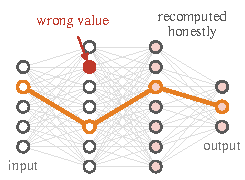
\includegraphics[width=0.47\columnwidth]{figures/overview_attack.pdf}}\hfill
  \subfloat[Defence: caught except with probability $2^{-\lambda}$]{%
    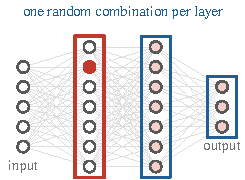
\includegraphics[width=0.47\columnwidth]{figures/overview_defence.pdf}}
  \caption{One tampered neuron whose later layers are recomputed honestly slips past a random path
  (a) but not past a check of every layer (b)}
  \label{fig:overview}
\end{figure}

\para{The attack.} A provider that wants to change an answer does not need a different model. It
runs the committed model, overwrites the value of a single neuron, and recomputes every later
layer honestly with the true weights. The resulting trace is inconsistent at exactly one site,
which a random path visits with probability $1/N$ (Figure~\ref{fig:overview}). On an MNIST network the tampered answer is
accepted with probability 99.6--99.8\%, and on the real OPT-6.7B, editing one feed-forward neuron
changes the next token for 40 of 40 prompts. Applied only to inputs that carry a trigger, the edit
is a backdoor in the serving code: the committed weights stay clean, and clean queries are
answered bit for bit as before. The attack also refutes a claim made for binary classifiers, for
which Anchuri et al.\ state that their analysis extends to full soundness. On a dog-vs-cat
ResNet-18, one changed penultimate neuron flips every test query and passes a path with
probability $511/512$. More paths do not help at a useful cost: catching the attack on Llama-2-7B
with probability $1-2^{-40}$ takes about 305{,}000 paths, which open about 13.7\,GB for a 64-token
prompt.

\para{A dichotomy for spot-checking.} The attack is an instance of a general limit. Because the
provider recomputes everything after the edit, the forged trace is the \emph{honest} trace of a
model that differs from the committed one in a single weight row. Suppose a verifier reads the
weights through a commitment in which each symbol it can query depends on at most $d$ rows, and
makes $q$ queries to a layer in expectation. We show that, when the other rows carry no information
about where the edit is, the verifier rejects the forgery at most as often as it could guess the
edited site in $qd$ tries (Theorem~\ref{thm:guess}). This holds for adaptive,
value-aware verifiers that read the whole claimed trace. In the worst case no verifier beats
uniform sampling: for every such verifier there is a ReLU network with a hidden layer of width $N$
and a single-neuron forgery, with every value in its natural range, that is accepted with
probability at least $1-qd/N$. Soundness $1-\varepsilon$ therefore requires
$qd \ge (1-\varepsilon)N$. Conversely, symbols that mix every row of a layer, such as random
linear combinations of its rows or the columns of a Reed--Solomon encoding of its weights, reach
$2^{-\lambda}$ with $O(\lambda)$ queries per layer, so the threshold is $\Theta(N)$ up to a factor
$O(\lambda)$ (Theorem~\ref{thm:dich}). That spot checks of an unencoded object catch a one-symbol
change only with probability about $q/N$ is
folklore~\cite{juels2007por,ergun2000spotcheckers,bghsv2006robust}. Our contribution is the
reduction that extends this limit to verifiers that read the whole trace, and its consequence: the
object that must be encoded is the model, not the trace. We apply the theorem to published schemes
under their own parameters (Table~\ref{tab:sok}). Most state probabilistic guarantees that their
sampling meets; for example, one audit of SLP's 70B configuration accepts an edited chunk with
probability 98.14\%. We do not call these schemes broken. Two claims exceed what the sampling
gives: the path protocol's full soundness for binary classifiers, and the negligible soundness
that TensorCommitments sets as its goal while choosing the checked layers by a rule that depends
only on the weights, so that an edit in a layer it does not choose always passes. We disclosed
these findings to the authors of the schemes before submission \todo{true only once the notices
scheduled for 15--19 Oct are sent; otherwise delete this sentence; summarise the replies in the
disclosure paragraph of Section~\ref{sec:sok}}.

\para{A defence that checks everything.} Since no verifier has a better worst-case guarantee than
uniform sampling, ours checks every weight operation of the model. The committed model is an int8
network whose results are bit-identical on the provider's GPU and on the client. With the output,
the provider sends the result of every weight operation. The verifier recomputes every operation
without weights, attention included, from these values, and checks each weight operation with a few
random linear combinations of its output rows (Freivalds' algorithm~\cite{freivalds1977}). A client
that does not hold the weights checks each combination against a Reed--Solomon-encoded,
Merkle-committed copy of them, in the style of Ligero~\cite{ligero}, and stores only a 32-byte root
per weight matrix. A tampered value anywhere in the network is then caught except with probability
$2^{-\lambda}$, and the protocol needs only a hash function and a linear code: no SNARK, no trusted
hardware and no trusted setup.

This design leaves four gaps, which we close. First, its soundness theorem assumes an
honestly computed commitment, and this assumption carries weight. A commitment that binds one model
on half of the encoded positions and a modified model on the other half lets the modified model
pass with probability about $2^{-t}$ per query for $t$ opened columns, which is $2^{-35}$ for the
smallest tree of Llama-2-7B. A one-time public setup proof, a proximity test that any client checks once,
removes the assumption (Section~\ref{sec:setup-proof}); for open-weight models anyone can instead
recompute the commitment from the checkpoint. Second, the Fiat--Shamir transcript binds the whole
computation, including every constant of the operations without weights, which avoids the weak
Fiat--Shamir pattern~\cite{bernhard2012pitfalls,dao2023weakfs}. Third, a generated response is
proved as one prefill. The verifier checks each generated token against the claimed logits before
it, either as the greedy choice or as the choice of an exact integer Gumbel-max sampler keyed by a
seed that the client picks, and neither rule adds a soundness term (Section~\ref{sec:gen}).
Fourth, we shrink the proof, which at long prompts consists mostly of the 32-bit results of the
weight operations. In V1 the provider sends instead the int8 value that the next operation reads,
and proves with a logUp-GKR~\cite{haboeck2022logup,papini2023logupgkr} that every hidden result
lies in the requantisation window of the value sent. The verifier knows each operation's input, so
these window conditions are linear in the committed weights, and the GKR's final claim reduces to
the existing folded rows and column check. V1 adds no commitment (Section~\ref{sec:v1}).

\para{Costs.} Beyond the forward pass, the prover's work without V1 grows with the model but not with
the input, and the prover is the protocol's strongest axis. Computing its column openings and folds with exact int8
tensor-core products instead of float64 makes it 3.7--4.3$\times$ faster on Llama-2 blocks on an
RTX~2080~Ti, and it proves a 256-token GPT-2 response to a 64-token prompt in 0.29\,s. On matched
models it is 46--32{,}000$\times$ faster than published zkSNARK provers \todo{L40S: final range; the
current one is from the pre-improvement L40S run}. The main cost is the proof. It carries the
results of every weight operation and so grows with the prompt: 325\,MB for a 64-token Llama-2-7B
query and 6.6\,GB at 2{,}048 tokens \todo{L40S}, against 183\,kB for zkLLM. V1 makes it
2.0--2.3$\times$ smaller at 2{,}048 tokens (the full OPT-1.3B: 2.07 to 0.96\,GB), at the price of
a GKR in the prover whose work grows with the number of results (OPT-125M at 2{,}048 tokens: 0.50
to 4.85\,s on the RTX~2080~Ti) and a CPU verifier that is 1.6--1.9$\times$ slower at that length \todo{L40S}. The verifier recomputes attention, so its cost
grows with the square of the prompt length. With eight CPU threads, a client that holds the weights
verifies a 64-token Llama-2-7B query in about 1.5\,s, against 3.5\,s for re-executing the model in
fp32, but at 2{,}048 tokens the two take about the same time, about 85\,s \todo{L40S/EPYC:
re-measure with the native attention kernel}. Our GPU claim decoder and fused exact attention kernel
make the streaming GPU verifier 2.7$\times$ faster on OPT-1.3B at that length \todo{L40S, full
models}. The protocol is not zero-knowledge: the
claims of $\lceil k/T\rceil$ queries of $T$ tokens reveal a weight matrix with rows of length $k$.
It therefore targets open-weight models served by an untrusted provider, the setting of
CommitLLM~\cite{commitllm2026} and of Gupta et al.~\cite{gupta2026private}. Finally, the provider
must serve the integer model. Moving SmoothQuant's per-channel scales~\cite{xiao2023smoothquant}
into the gains of the integer LayerNorm brings its WikiText-2 perplexity within a factor of 1.03 of
fp32 on OPT-125M and OPT-1.3B, from 1.17 and 1.11, without changing any operation that the
protocol checks \todo{OPT-6.7B and Qwen3-4B with smoothing}.

\para{Contributions.} We make the following contributions.
\begin{itemize}
  \item \emph{An attack on spot-checking proofs of inference} (Section~\ref{sec:attack}): a
  single-site edit followed by honest recomputation, measured on image classifiers and on the real
  OPT-6.7B. It passes the path protocol of~\cite{anchuri2026verifiable} with probability $1-1/N$
  per path and refutes its full-soundness claim for binary classifiers.
  \item \emph{A dichotomy theorem and a systematisation} (Section~\ref{sec:sampling},
  Table~\ref{tab:sok}): against honest recomputation, a verifier that reads the weights through a
  commitment of locality $d$ needs $qd \ge (1-\varepsilon)N$ per layer, which mixing commitments
  meet with $O(\lambda)$ queries. We apply it to nine published inference-verification schemes.
  \item \emph{A fully sound Freivalds-based protocol that needs only a hash function and a linear
  code}
  (Sections~\ref{sec:defence}--\ref{sec:v1}), sound against an untrusted committer, with a
  Fiat--Shamir transcript bound to the whole computation, greedy and sampled generation, and V1,
  which halves the proof at long prompts.
  \item \emph{An evaluation} (Section~\ref{sec:results}) of the attack and the defence on image
  classifiers and language models up to 13B parameters, with re-execution baselines, the quality
  of the integer models, and comparisons with published systems \todo{L40S}.
\end{itemize}

% =====================================================================================
\section{Related Work}
\label{sec:related}

\para{zkSNARK proofs of inference.} A long line of work compiles neural networks into succinct
proofs. For CNNs these include sum-check and GKR provers~\cite{gkr} such as zkCNN~\cite{zkcnn},
zkPyTorch~\cite{zkpytorch} and VerfCNN~\cite{verfcnn}, and pairing- or Plonk-based systems such as
vCNN~\cite{vcnn}, ZEN~\cite{zen}, ZENO~\cite{zeno}, ZKML~\cite{zkml}, EZKL~\cite{ezkl} and
Bionetta~\cite{bionetta}; Mystique~\cite{mystique} is an interactive, VOLE-based alternative. For
language models they include zkLLM~\cite{zkllm}, zkGPT~\cite{zkgpt}, DeepProve~\cite{deepprove},
ZKTorch~\cite{zktorch}, Jolt Atlas~\cite{joltatlas} and the full mode of NanoZK~\cite{nanozk}. They
give computational soundness with proofs of under a kilobyte to tens of megabytes, and many of them
hide the weights. Their provers are far slower than inference. zkLLM takes 620\,s on an A100 for a
2{,}048-token Llama-2-7B prompt, with a 183\,kB proof~\cite{zkllm}; ZKTorch takes 44\,min for one
Llama-2-7B token~\cite{zktorch}; DeepProve takes 34\,s for a 64-token GPT-2 prompt on a 16-core
CPU~\cite{deepprove}. DeepProve and zkAgent~\cite{zkagent} prove a generated sequence in one pass
over the prompt and the output, which is also how we prove generation. These systems prove
non-linear operations with lookup arguments, such as zkLLM's tlookup and the
logUp-GKR~\cite{papini2023logupgkr} that DeepProve uses. V1 borrows this
machinery for one narrow purpose, to show that hidden results lie in their requantisation windows.
The weight products still go through Freivalds' check against the existing commitment, and no
activation is committed. Hollow-LLM~\cite{hollowllm} observes that a valid proof over committed
private weights does not establish that the provider performed the computation of a model of the
declared size, since weights with a degenerate algebraic structure keep the declared shapes but are
cheap to evaluate. Our protocol shares this limitation for private weights; for open weights the
commitment is recomputed from the checkpoint. Our protocol gives up the zkSNARKs' small proofs and weight privacy in exchange for a prover that
is orders of magnitude faster.

\para{Spot-checking and sampling.} Anchuri et al.~\cite{anchuri2026verifiable} spot-check random
paths through a committed trace and prove other-model soundness through trace separation.
SLP~\cite{slp} commits every chunk boundary and proves a random subset of chunks with a SNARK.
CommitLLM's routine audit~\cite{commitllm2026} opens 10 of 80 layers at one token of an audited
response. TensorCommitments~\cite{tensorcommitments} and NanoZK's audit mode~\cite{nanozk} check a
subset of layers, SPEX~\cite{spex} re-executes with a fixed probability, and
IMMACULATE~\cite{immaculate} audits a fraction of requests. TOPLOC~\cite{toploc} and
SVIP~\cite{svip} fingerprint hidden states and target model, prompt or precision substitution.
Verde~\cite{verde}, opML~\cite{opml} and TAO~\cite{tao} are optimistic: an answer stands unless a
party that re-runs the model disputes it, so they rely on an honest party that re-runs every query.
Table~\ref{tab:sok} places these designs under our theorem. SLP and CommitLLM themselves describe
the edit-then-recompute strategy~\cite{slp,commitllm2026}, and the calculation behind it is
classical. It underlies proofs of retrievability and of data
possession~\cite{juels2007por,ateniese2007pdp}, it is why spot-checkers certify only
closeness~\cite{ergun2000spotcheckers}, and it is why PCPs of proximity guarantee only that their
input is close to the language while holographic proofs encode their
input~\cite{bghsv2006robust,bfls1991,chiesa2020fractal}. Our theorem turns this calculation into a
bound for adaptive, value-aware verifiers that read the whole trace; its tight case is the optimal
search for a hidden object~\cite{kadane1971}. Proof-of-Learning~\cite{jia2021pol}, which checks the
largest weight updates of a training run, is a precedent for value-dependent sampling being
gamed~\cite{zhang2022pol,fang2023pol}.

\para{Trusted hardware.} Slalom~\cite{slalom} checks the linear layers of a GPU computation from
inside an SGX enclave with Freivalds' algorithm, optionally with a precomputed secret challenge.
TwinShield~\cite{twinshield} and VeriAttn~\cite{veriattn} extend enclave-based checking to
attention, and VeriAttn accepts results within a tolerance. These designs are fast, but their
guarantee rests on the enclave and its vendor. Our protocol needs no trusted hardware, and its exact
integer semantics leaves no tolerance in which to hide a change.

\para{Freivalds-based checks.} SafetyNets~\cite{safetynets} uses interactive proofs
for networks with quadratic activations, and ZKML~\cite{zkml} uses Freivalds' check for linear layers
inside a SNARK. Maverick~\cite{maverick} checks every linear layer of a language model with sparse
Freivalds checks against a code-encoded copy of the weights that the client stores. Gupta et
al.~\cite{gupta2026private} run Freivalds' check in the exponent of a group, against verification
data that the model owner generates with secret randomness, for a client that outsources inference
to two non-colluding servers. CommitLLM~\cite{commitllm2026} checks int8 language models with secret
Freivalds vectors precomputed from the weights, at 12--14\% serving overhead, and audits attention
without verifying it. LAMP~\cite{lamp} lets a verifier that holds only a commitment check one matrix
product, with Freivalds' check and Reed--Solomon proximity testing inside a Groth16 SNARK. Our column
check is that of the Ligero and Brakedown commitments~\cite{ligero,brakedown}, and our setup proof
is a one-time proximity test in the style of Ligero. Among zkSNARKs, DeepProve's hash-based
configuration commits with BaseFold~\cite{basefold}.

\para{Where we fit.} We keep the setting of Anchuri et al., a client that holds only a commitment to
the weights, and replace the sampled check, which needs $(1-\varepsilon)N$ paths per layer for
soundness $1-\varepsilon$ (Theorem~\ref{thm:dich}), with a check of every weight operation. Each of
the protocols above that avoids a SNARK needs more than a cryptographic commitment: Slalom an
enclave, Maverick an encoded copy of the weights, CommitLLM a secret derived from them, and Gupta
et al.\ public data that grows with every matrix and is generated with secret randomness. zkSNARKs
that verify against a Merkle root, such as DeepProve with BaseFold, need no trusted setup but prove
far more slowly. To our knowledge, ours is the first Freivalds-based proof of inference that is
fully sound for complete transformers, attention included, whose client needs no enclave, no stored
copy of the weights and no weight-derived secret. It uses no SNARK, only a hash function and a
linear code, and with the setup proof it does not trust the party that computes the commitment.
